\insertbigimage{figures/block_diagram.pdf}{Block diagram of the system}{block_diagram}

\section{System Design Overview}

The system was designed around the RP2040 microcontroller, acting as the central 
processing unit for interfacing with a variety of sensors and control devices. 
The design incorporates the SF-5M sap flow sensor, LT-1T leaf temperature sensor, 
and MT-603 load cell to measure various environmental parameters. Each of these 
sensors use different communication protocols, requiring careful consideration of 
power requirements, signal integrity, and communication compatibility. A photo 
of the board is shown in \cref{board_photo} while \cref{block_diagram} 
shows an overview of all the communication systems involved in the design.

\begin{figure}
    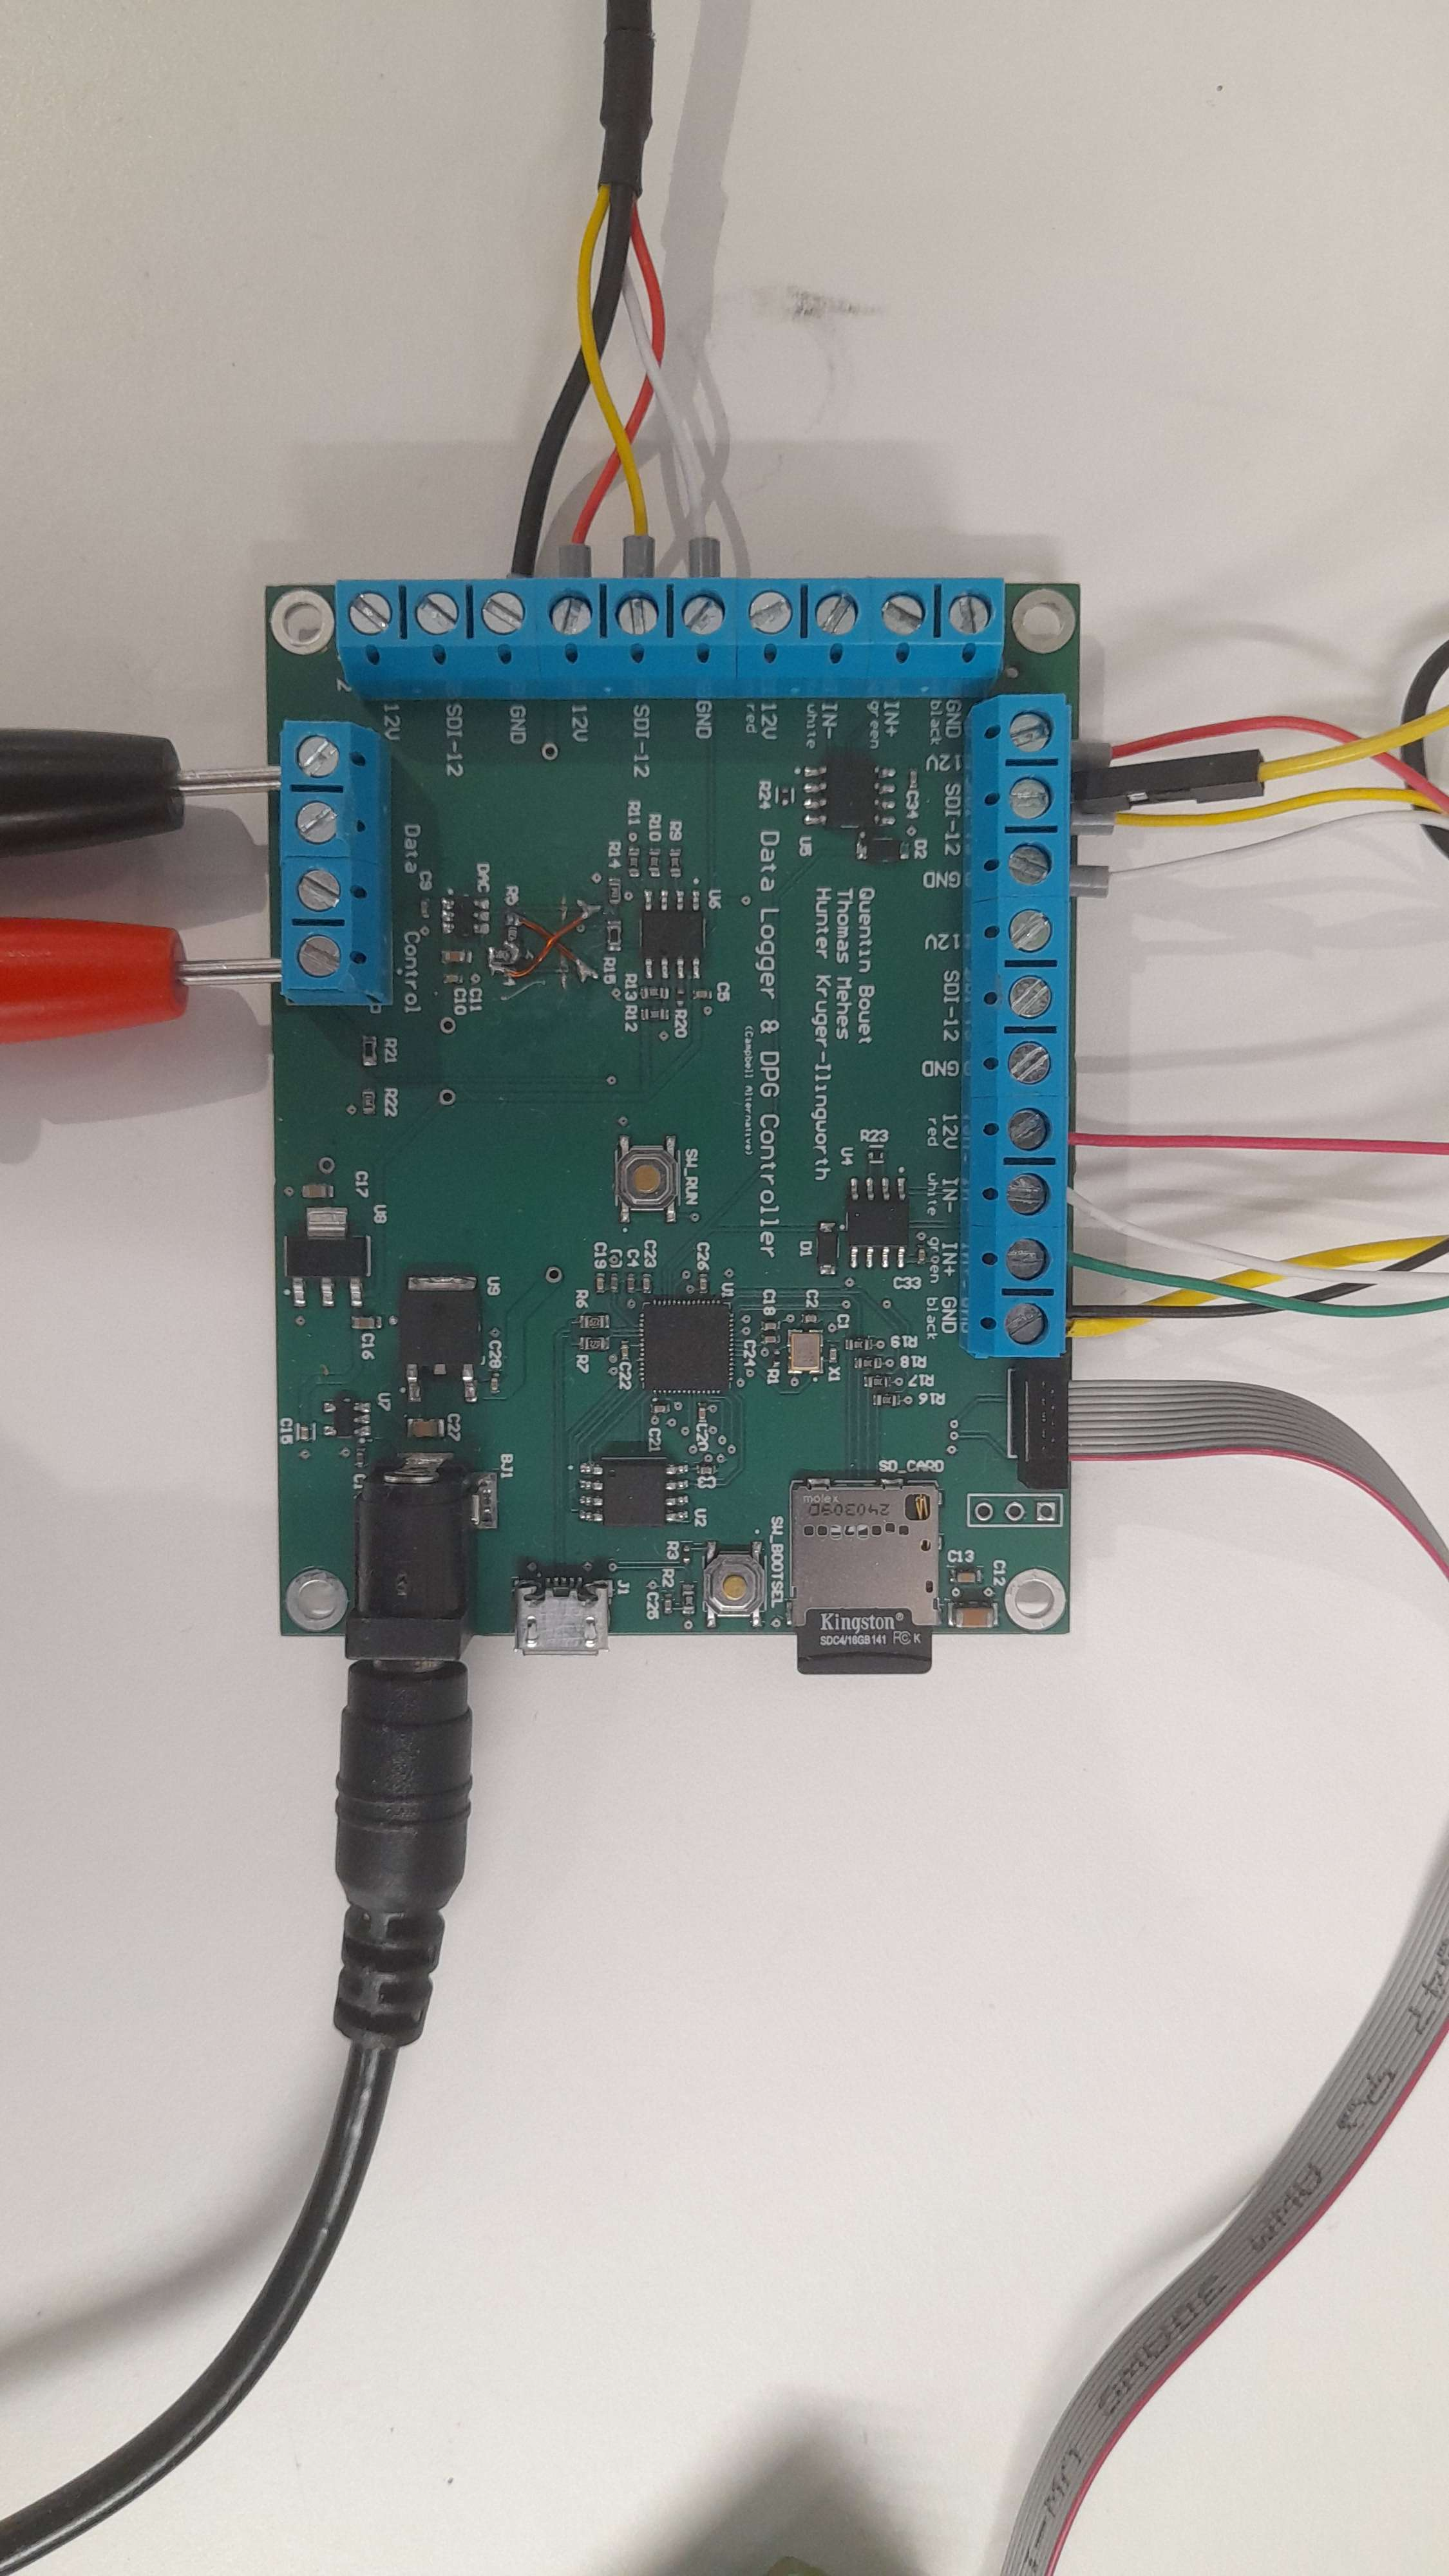
\includegraphics[width=0.4\linewidth]{figures/board_photo.jpg}
    \caption{Photo of Board}
    \label{board_photo}
\end{figure}

\begin{figure}
    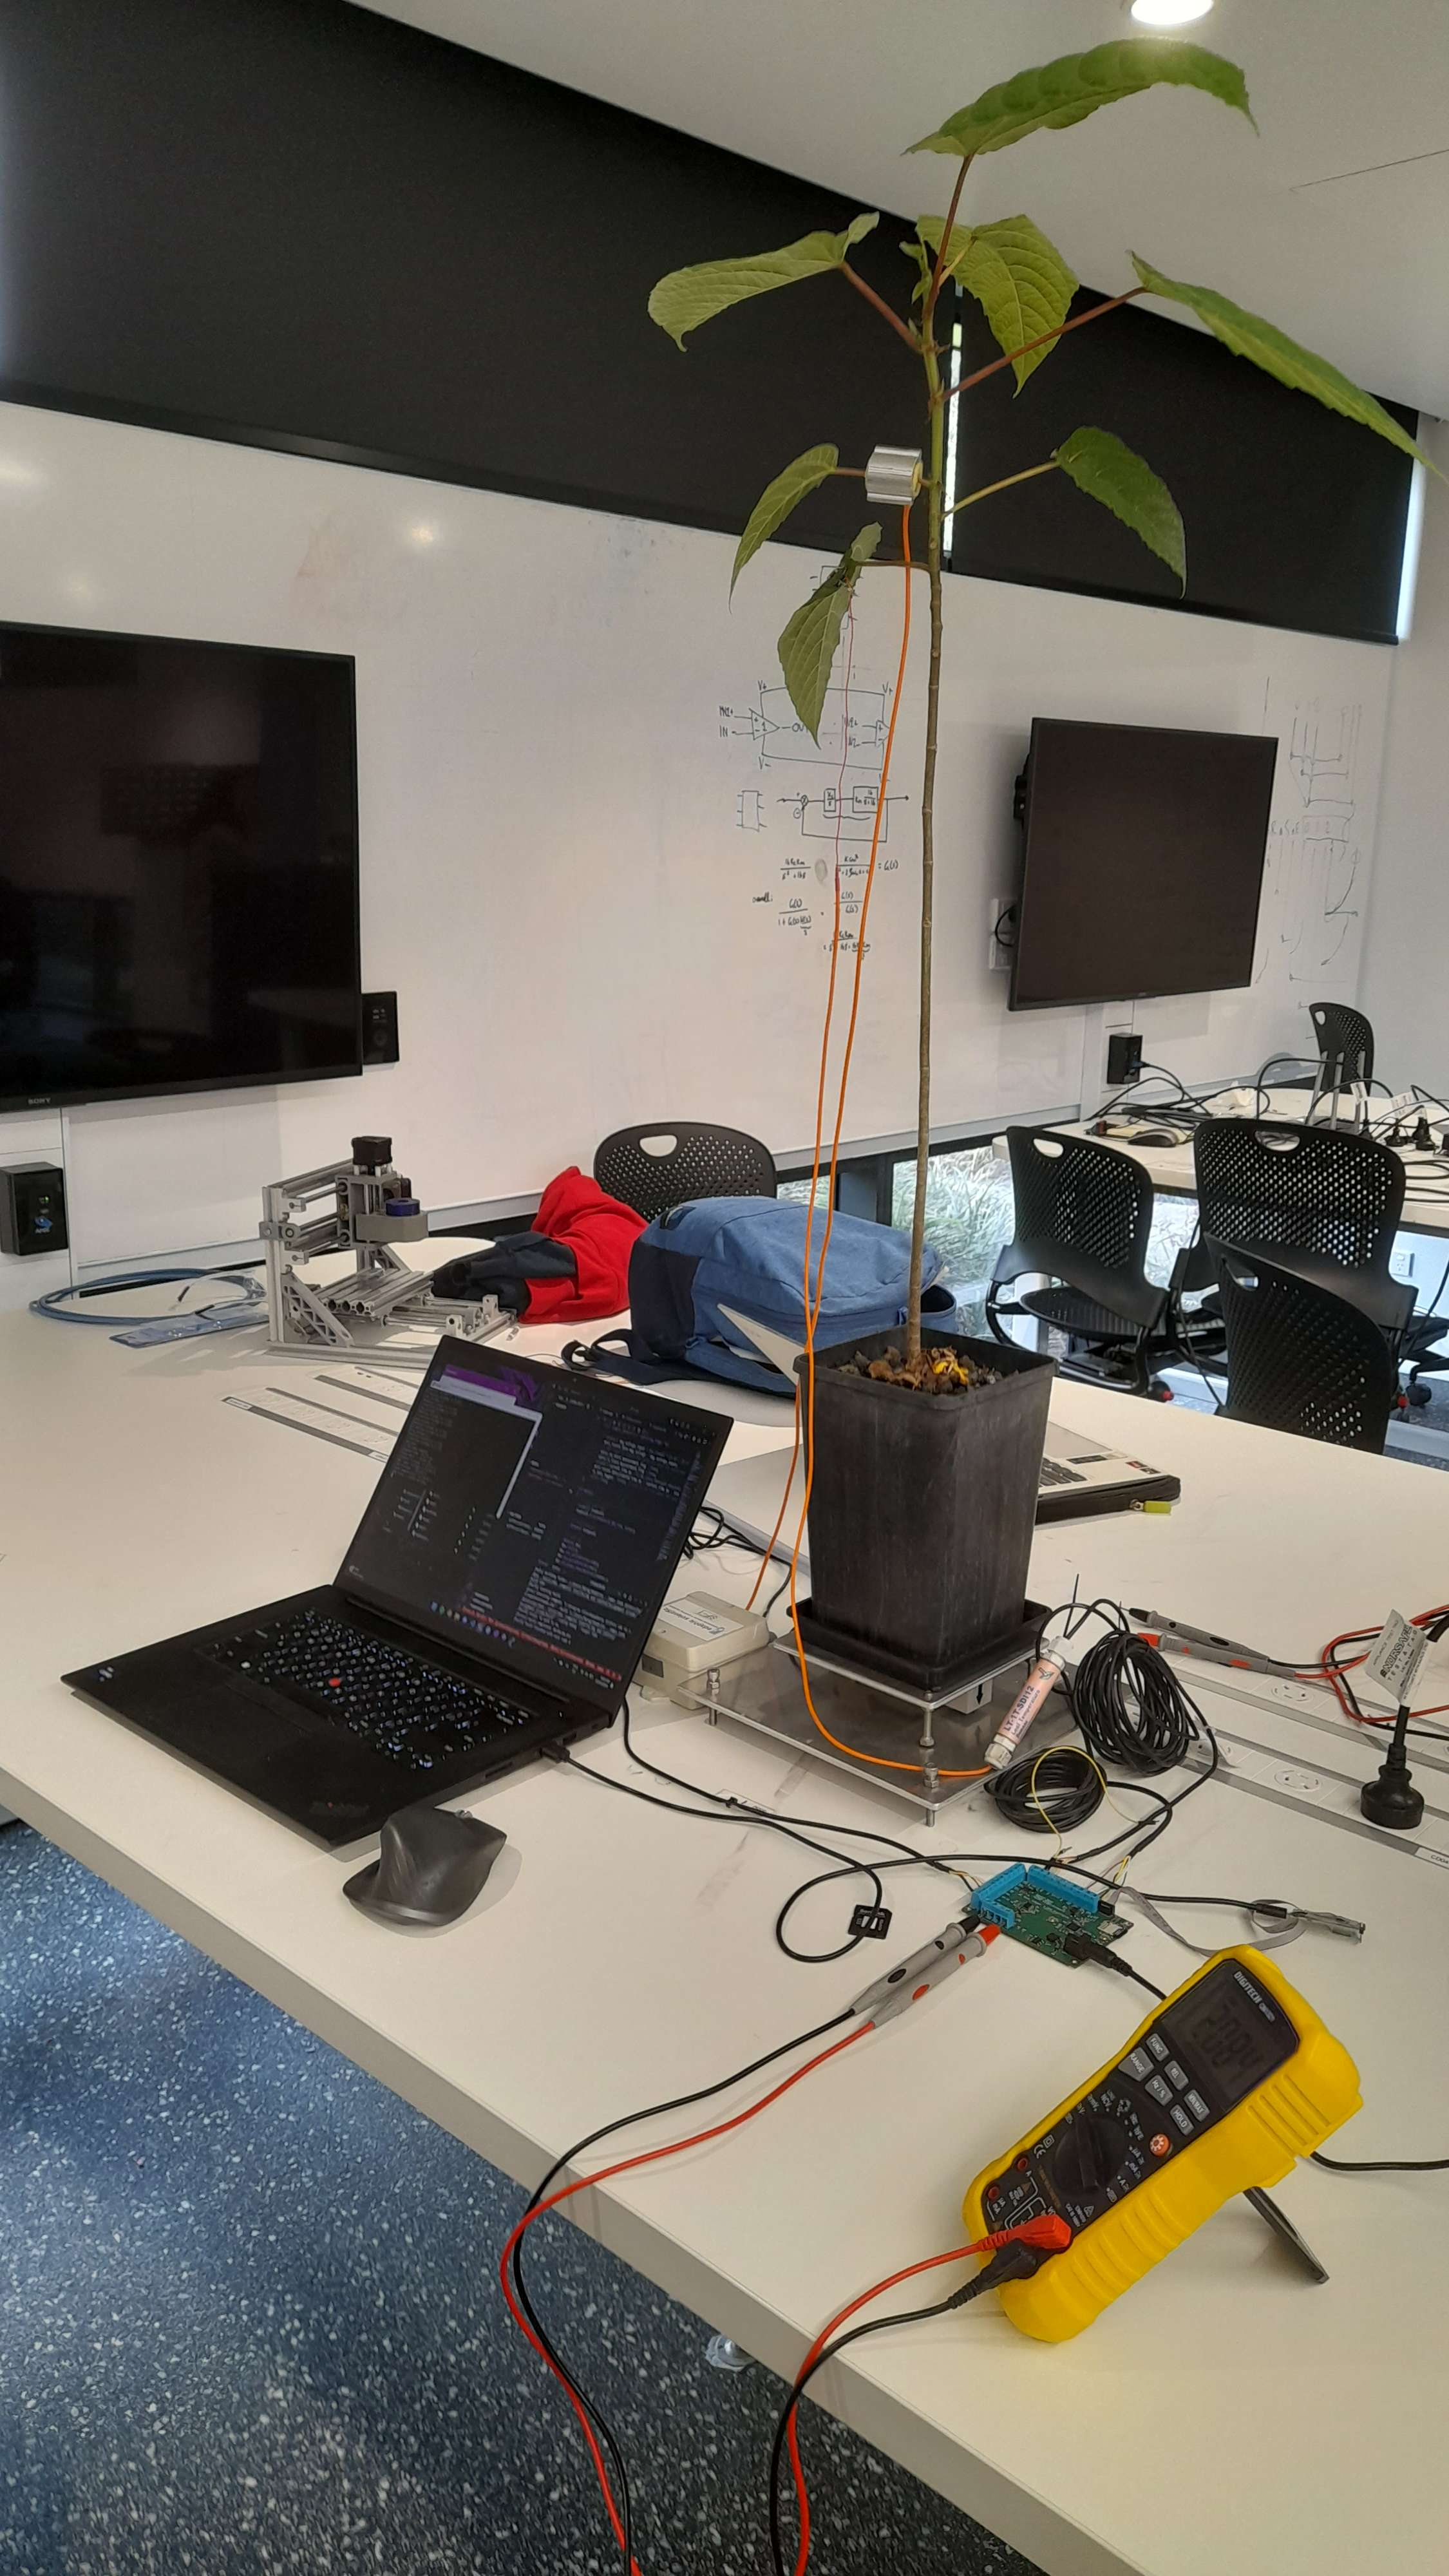
\includegraphics[width=0.4\linewidth]{figures/system_setup_1.jpg}
    \caption{Photo of System Setup}
    \label{system_photo}
\end{figure}

